\section{Classification of tweets}
One of the similar projects is described in the article "Entity Extraction, Linking, Classification, and Tagging for Social Media: A Wikipedia-Based Approach"\cite{entityextraction}. The initial problem is a content analysis problem where they wanted to let the computer understand what the tweets are about and then sort them based on their content. The chosen solution to the problem was to use automatic classification of the tweets, where the tweets were categorized by their content. This problem is very similar to our problem because both the problems are based on understanding texts by recognizing keywords that provide information of categories, i.e., what the tweets are about.

The article describes the categorization as the machine learning process where tweets with similar content are placed in the same class. The authors chose to use Wikipedia as their knowledge base (a repository for information) for finding information of the different categories. The reasons given for why they chose Wikipedia are similar to our reasons;  it is the largest online encyclopedia, it is based on volunteering which means that it is rapidly updated, and it is constantly crawling which is important since it is an advantage to have a fresh, dynamic and timely knowledge base. 

The processing of the tweets required a lot of preprocessing before they could be classified content, especially since tweets are quite sort (max 160 characters).  The preprocessing of the tweets contained several steps before the actual categorization could start, including language detection, cleaning of the tweets (removing everything that is not text), and a tokenizing process (separating sentences into tokens, where a token is defined as a sequence of characters, usually normal words). The described preprocessing is similar to the preprocessing intended for our content analysis because the classifier will only find the keywords if they are an exact match. The classifier depend on tokenizing and cleaning of the words in the text to make them similar to keywords in the keyword list.  

The described tweet classification required some structure to keep information of the tweets and their possible categories. The solution was to create a structure of mentions where a mention is defined on the form ($m_{i}$, $n_{i}$, $s_{i}$), where $m_{i}$ is the string in the tweet we refer to, $n_{i}$ is the node in the knowledge base, and  $s_{i}$ is the< score of the node. All tokens with a connection to the knowledge base (i.e., Wikipedia) were considered relevant, while the others were removed to reduce the complexity. The structure of mentions could be too complex for our case with collections of texts since each text can be much longer than 160 characters, but the idea of keeping track of possible categories is the same. 

A scoring function was used for deciding categories for the tweets, where all the mentions were filtered and some hand-crafted rules were applied. Our project would also need some function to decide what categories are relevant if many categories are proposed. 


\subsection{Evaluation of the classification of tweets}
Evaluation is one of the most important part of a categorization process because it tells if the classification behaves as desired. Classification is, as already mentioned, difficult to evaluate and it was therefore quite useful to look at the evaluation part of the classification of tweets.

The authors argued that the computer classification should be compared by classification done by humans, so that the \textit{predicted} result could be compared with the \textit{correct} result. The problem is that it is very time consuming for humans to classify, so the evaluation was done by sampling 500 tweets. Of these tweets were 477 manually identified by people to give them tags which were compared by the classifier's tags. 

Figure \ref{fig:classification_entities} shows the results of the evaluation phase of the classification. The measures for each tag are P (precision: fraction of retrieved tweets that are relevant), R (recall: fraction of relevant tweets that were tagged) and F1 (F1-score: measure of accuracy, given as $ F_1 = 2 \cdot \frac{\mathrm{precision} \cdot \mathrm{recall}}{\mathrm{precision} + \mathrm{recall}}$). It is interesting to look at the results from the evaluation because they give a good indication on which subjects are difficult to classify. The results show that people and locations are easy to classify, while music is more difficult. This could be because music might contain common words that are dropped from the knowledge base or does not provide useful information while name of locations are easy to recognize for the classifier. 
%One of the most important steps of classifying is the evaluation phase. Evaluation of classifying should be done by humans. Someone will have to look through the results and see how well the classification has been done by comparing the \textit{correct} result with the \textit{predicted} result.

%The article concludes that the tweets that were easiest to classify were about people (see Figure \ref{fig:classification_entities}). This is probably because famous people have their own Wikipedia page, which is easy to match the tweet. The most difficult, on the other hand, was products which seldom have their own page  if the tweet is very specific. 


\begin{figure}[H]
\centering
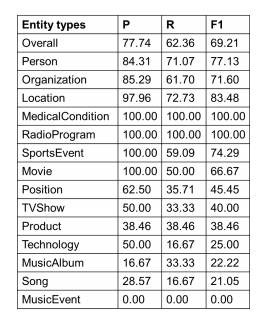
\includegraphics[height=8cm]{Classification_entities}
\caption{The accuracy of the system for extraction and linking.}
%P is the precision, R is the recall and $F_{1}$ is the $F_{1}$-score.} %linking\footnote{\url{http://pages.cs.wisc.edu/~anhai/papers/doctagger-vldb13.pdf, page 8}}}
\label{fig:classification_entities}
\end{figure}